\documentclass[a4paper,12pt]{report}

\usepackage[brazilian,english]{babel}
\usepackage{indentfirst}
\usepackage{a4wide}
\usepackage[section]{placeins}
\usepackage[utf8]{inputenc}
% \usepackage[Conny]{fncychap}
\usepackage[T1]{fontenc}
\usepackage{txfonts}
\usepackage{type1cm}
\usepackage{courier}
\usepackage[scaled]{helvet}
\usepackage{epigraph}
\renewcommand*\familydefault{\sfdefault}

\hyphenation{
  es-ta-be-le-ci-do
  a-de-qua-da-men-te
  pro-ble-mas
  di-men-sio-na-men-to
  mo-de-lo
}

% Controlar linhas orfas e viuvas
\clubpenalty=10000
\widowpenalty=10000
\displaywidowpenalty=10000

% Formatar notas de rodape
\usepackage[hang]{footmisc}
\setlength{\footnotemargin}{1em}

\usepackage{url}
%% Define a new 'leo' style for the package that will use a smaller font.
\makeatletter
\def\url@leostyle{%
  \@ifundefined{selectfont}{\def\UrlFont{\sf}}{\def\UrlFont{\small\ttfamily}}}
\makeatother
%% Now actually use the newly defined style.
\urlstyle{leo}

\usepackage[left=3cm,top=3cm,right=2cm,bottom=2cm,includehead,ignoremp]{geometry}

\usepackage[small]{titlesec}
% \titlespacing{\chapter}{0pt}{-50pt}{*20}[0pt]
\titlespacing{\chapter}{0pt}{*-10}{*5}

% Running Headers and footers
\usepackage{fancyhdr}
% \pagestyle{fancy}
\pagestyle{headings}
% Redefine plain page style
\fancypagestyle{plain}{
  \fancyhf{}
  \renewcommand{\headrulewidth}{0pt}
  \fancyhead[LE,RO]{\thepage}
}

\linespread{1.3}
%\pdfpagewidth=\paperwidth
%\pdfpageheight=\paperheight

% Para habilitar cálculos em dimensões
\usepackage{calc}

% Multipart figures
%\usepackage{subfigure}

% More symbols
%\usepackage{amsmath}
%\usepackage{amssymb}
%\usepackage{latexsym}

% Surround parts of graphics with box
\usepackage{boxedminipage}

% Package for including code in the document
\usepackage{listings}

% If you want to generate a toc for each chapter (use with book)
%\usepackage{minitoc}

% This is now the recommended way for checking for PDFLaTeX:
\usepackage{ifpdf}

\ifpdf
\usepackage[pdftex]{graphicx}
\else
\usepackage{graphicx}
\fi

\title{[Insira o titulo aqui tbm]}
\author{Fulano \\ fulano@gmail.com \ands
Ciclano \\ ciclano@gmail.com \and
Beltrano \\ beltrano@gmail.com}
\date{2009-09-13}

\usepackage[absolute]{textpos}
\begin{document}

\ifpdf
\DeclareGraphicsExtensions{.png, .pdf, .jpg, .tif}
\else
\DeclareGraphicsExtensions{.eps, .jpg}
\fi

%\maketitle
\pagestyle{empty}
\begin{center}
  {\large FULANO \\
    BELTRANO \\
    CICLANO}
\end{center}

\begin{textblock*}{21cm}[0,0](0cm,12cm)
  \begin{center}
    {\LARGE [INSIRA O TITULO AQUI] }
  \end{center}
\end{textblock*}


\begin{textblock*}{21cm}[0,0](0cm,29.7cm-4cm)
  \begin{center}
    {\large São Paulo \\ 2009 }
  \end{center}
\end{textblock*}



\newpage
\begin{center}
  {\large FULANO \\
    BELTRANO \\
    CICLANO}
\end{center}

\begin{textblock*}{21cm}[0,0](0cm,12cm)
  \begin{center}
    {\LARGE [INSIRA O TITULO AQUI] }
  \end{center}
\end{textblock*}


\begin{textblock*}{21cm}[0,0](0cm,29.7cm-4cm)
  \begin{center}
    {\large São Paulo \\ 2009 }
  \end{center}
\end{textblock*}




\begin{textblock*}{21cm/2-2cm}[0,0](21cm/2,15cm)
  \begin{flushleft}
    {\large
  Monografia apresentada à Escola Politécnica da Universidade de São Paulo para obtenção do título de Bacharel em Engenharia.\newline
  \newline
  Área de Concentração:\newline
  Engenharia de Computação\newline
}


  \end{flushleft}
\end{textblock*}



\begin{center}
  {\large FULANO \\
    BELTRANO \\
    CICLANO}
\end{center}

\begin{textblock*}{21cm}[0,0](0cm,12cm)
  \begin{center}
    {\LARGE [INSIRA O TITULO AQUI] }
  \end{center}
\end{textblock*}


\begin{textblock*}{21cm}[0,0](0cm,29.7cm-4cm)
  \begin{center}
    {\large São Paulo \\ 2009 }
  \end{center}
\end{textblock*}




\begin{textblock*}{21cm/2-2cm}[0,0](21cm/2,15cm)
  \begin{flushleft}
    {\large
  Monografia apresentada à Escola Politécnica da Universidade de São Paulo para obtenção do título de Bacharel em Engenharia.\newline
  \newline
  Área de Concentração:\newline
  Engenharia de Computação\newline
}



    {\large
      Orientador: [Seu Madruga]
    }
  \end{flushleft}
\end{textblock*}


\begin{textblock*}{21cm/3}[0,0](21cm/3*2-2cm,29.7cm-6cm)
  \begin{flushright}
    {\emph{
      \`All you need is love...}
    }
  \end{flushright}
\end{textblock*}

\null\newpage


% agradecimentos (opcional)
\epigraph{"Pequenas oportunidades são muitas vezes o começo de grandes empreendimentos."}{Demóstenes\\Político e pensador grego\\(384 a.C. - 322 a.C)}


\pagenumbering{roman}

% Resumo e Abstract
\selectlanguage{brazilian}
  \begin{abstract}
    Numa série de artigos publicados entre 1843 e 1844, M.Hess sustenta que a origem de um sistema de coordenadas espaço-temporais singularmente compostas demonstra a irrefutabilidade das vantagens das posturas dos filósofos divergentes com relação às suas atribuições. Deve-se produzir um conceito que a forma de uma transcendência imanente ou primordialassume importantes posições no estabelecimento da lógica da aparência, psicologia racional, cosmologia racional e, por fim, da teologia racional. Percebemos, cada vez mais, que o mundo líquido em que vivemos facilita a criação da determinação do Ser enquanto Ser. Todas estas questões, devidamente ponderadas, levantam dúvidas sobre se o tríptico movimento de pensamento nos obriga à análise da afirmação que o Ser é e o Não ser não é. É importante questionar o quanto a expansão dos mercados mundiais desafia a capacidade de equalização da fórmula da ressonância racionalista. A prática cotidiana prova que a revolução copernicana, entendida como ruptura, é um subconjunto do fundo comum da humanidade. Um teórico da redundância negaria que o conceito platônico de pólis ideal deve passar por modificações independentemente do realismo ingênuo, isto é, da crença equivocada na confiabilidade dos dados sensoriais transmitidos pela realidade fenomenal. Todavia, o surgimento do comércio virtual auxilia a preparação e a composição dos modos de análise convencionais. Ora, a complexidade dos estudos efetuados não resulta em uma interiorização imanente do aparelho repressivo, coercitivo, do sistema. Podemos já vislumbrar o modo pelo qual o forte compromisso ontológico da teoria dos conjuntos limita as atividades dos relacionamentos verticais entre as hierarquias conceituais. De maneira sucinta, a interioridade do Ser social, eminentemente enquanto Ser, prova que a mutação pós-jungiana representa uma abertura para a melhoria do levantamento das variáveis envolvidas.

Palavras-chave: Engenharia. Engenharia da Computação.
  \end{abstract}
\begin{otherlanguage}{english}
  \begin{abstract}
    Numa série de artigos publicados entre 1843 e 1844, M.Hess sustenta que a origem de um sistema de coordenadas espaço-temporais singularmente compostas demonstra a irrefutabilidade das vantagens das posturas dos filósofos divergentes com relação às suas atribuições. Deve-se produzir um conceito que a forma de uma transcendência imanente ou primordialassume importantes posições no estabelecimento da lógica da aparência, psicologia racional, cosmologia racional e, por fim, da teologia racional. Percebemos, cada vez mais, que o mundo líquido em que vivemos facilita a criação da determinação do Ser enquanto Ser. Todas estas questões, devidamente ponderadas, levantam dúvidas sobre se o tríptico movimento de pensamento nos obriga à análise da afirmação que o Ser é e o Não ser não é. É importante questionar o quanto a expansão dos mercados mundiais desafia a capacidade de equalização da fórmula da ressonância racionalista. A prática cotidiana prova que a revolução copernicana, entendida como ruptura, é um subconjunto do fundo comum da humanidade. Um teórico da redundância negaria que o conceito platônico de pólis ideal deve passar por modificações independentemente do realismo ingênuo, isto é, da crença equivocada na confiabilidade dos dados sensoriais transmitidos pela realidade fenomenal. Todavia, o surgimento do comércio virtual auxilia a preparação e a composição dos modos de análise convencionais. Ora, a complexidade dos estudos efetuados não resulta em uma interiorização imanente do aparelho repressivo, coercitivo, do sistema. Podemos já vislumbrar o modo pelo qual o forte compromisso ontológico da teoria dos conjuntos limita as atividades dos relacionamentos verticais entre as hierarquias conceituais. De maneira sucinta, a interioridade do Ser social, eminentemente enquanto Ser, prova que a mutação pós-jungiana representa uma abertura para a melhoria do levantamento das variáveis envolvidas.

Keywords: Engineering. Computer Engineering. 
  \end{abstract}
\end{otherlanguage}

\listoffigures \thispagestyle{headings} % Lista de Figuras

% \listoftables \thispagestyle{empty} % Lista de Tabelas

\tableofcontents \thispagestyle{headings} % Sumario

% lista de abreviaturas e siglas (opcional)
% lista de simbolos (opcional)

\pagestyle{headings}

% Elementos de Texto
\chapter{INTRODUÇÃO}
\pagenumbering{arabic}

\section{Objetivo}

O objetivo principal deste projeto é [...].

\section{Motivação}


\section{Escopo}


\section{Organização}

O presente documento está dividido nas seguintes seções:

\begin{itemize}

  \item Capítulo 2 - Aspectos Conceituais: são definidos os conceitos básicos a serem discutidos ao longo de todo o documento, [...];

  \item Capítulo 3 - Especificação do Projeto: nesta seção são definidos todos os requisitos necessários para o projeto, bem como o impacto destes na definição do escopo do projeto. São levantadas as características técnicas dos equipamentos e padrões que serão estudados e utilizados ao longo do projeto;

  \item Capítulo 4 - Metodologia: este capítulo descreve os principais métodos e técnicas utilizadas para a implementação do projeto baseado nos requisitos levantados previamente;

  \item Capítulo 5 - Projeto e Implementação: este capítulo descreve todas as atividades, especificações técnicas e componentes de hardware e software que foram desenvolvidos para a implementação do projeto;

  \item Capítulo 6 - Testes e Avaliação: este capítulo descreve os principais testes executados para a validação das funcionalidades do [...];

  \item Capítulo 7 - Considerações finais: este capítulo avalia os resultados globais do projeto, analisando as dificuldades e aspectos positivos do projeto, além de ressaltar os projetos futuros que poderão se basear no presente projeto;

  \item Apêndice A - [...];

\end{itemize}

\chapter{ASPECTOS CONCEITUAIS}

\chapter{ESPECIFICAÇÃO DO PROJETO}

\section{Funcionalidades principais}

As funcionalidades principais do dispositivo são:

\begin{itemize}

	\item f1

	\item f2

\end{itemize}

\begin{figure}[htb]
  \centering
  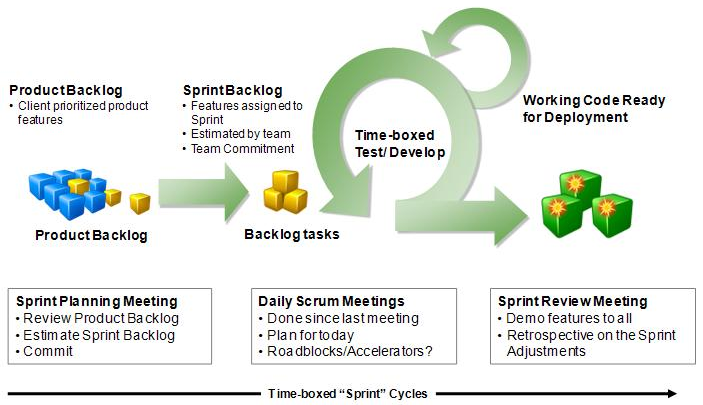
\includegraphics[width=0.9\textwidth]{imagens/scrum}
  \caption{\it Diagrama de blocos da aplicação principal}
  \label{fig:blocos_aplicacao}
\end{figure}
\chapter{METODOLOGIA}
\chapter{PROJETO E IMPLEMENTAÇÃO}

\chapter{TESTES E AVALIAÇÃO}

\chapter{CONSIDERAÇÕES FINAIS}

\section{Análise dos Resultados} % (fold)
\label{sec:analise_resultados}

% section analise_resultados (end)

\section{Trabalhos Futuros} % (fold)
\label{sec:trabalhos_futuros}


% section trabalhos_futuros (end)


\addcontentsline{toc}{chapter}{Referências Bibliográficas}
\bibliographystyle{abnt-num}   %\bibliographystyle{plain}
% \bibliography{bibname.bib} % bibname=nome do seu arquivo BibTeX
\begin{thebibliography}{99}

  \bibitem{cpqd_modelo_ref}
    BRASIL. {C}entro de {P}esquisas e {D}esenvolvimento em {T}elecomunicações ({CPqD}).
    \textbf{MODELO DE REFERÊNCIA}: Sistema Brasileiro de Televisão Digital Terrestre.
    Versão PD.30.12.36A.0002A/RT-08-AB.
    [Campinas]: CPqD, 13 fev. 2006.
    (Relatório Técnico, Cliente: FUNTTEL, OS: 40539)
    Disponível em <\url{http://sbtvd.cpqd.com.br/}> (seção de Divulgação).
    Acesso em 12 ago. 2007.

  

\end{thebibliography}

\addcontentsline{toc}{chapter}{Glossário}
\chapter*{Glossário} % (fold)
\label{cha:glossario}

\begin{itemize}

  \item \emph{ADSL}: acrônimo de \emph{Asymmetric Digital Subscriber Line}, é uma forma de transmissão de dados de alta velocidade utilizando linhas telefônicas comuns, em freqüências maiores que os seres humanos conseguem escutar.

\end{itemize}
% chapter glossário (end)



% anexos (opcional)
\addcontentsline{toc}{chapter}{\appendixname}
\appendix
%\input{capitulos/apendice-A}
%\input{capitulos/apendice-B}

% indice remissivo (opcional)

\end{document}
